\section{Architekturmuster}\label{sec:architekturmuster}

\textbf{Architekturmuster} sind wie Analysemuster\footnote{
    s. Abschnitt~\ref{sec:analysemuster}
} \textbf{Lösungsskizzen} verallgemeinerter Architekturprobleme.

\noindent
Im Folgenden werden zwei Muster vorgestellt.

\subsection{Client-Server}

\subsubsection*{Problem in seinem Kontext}
\begin{itemize}
    \item Mehrere Nutzer arbeiten gleichzeitig und verteilt an mehreren Rechnern
    \item es wird auf dieselben Daten zugegriffen
    \item Daten werden ausgetauscht
    \item gemeinsame Daten bzw. Arbeitsabläufe werden synchronisiert
    \item eine \textit{direkte Kommunikation} zwischen den Arbeitsplätzen ist \textit{nicht erwünscht}, bspw. aus Sicherheitsgründen oder wegen der hohen Anzahl der Nutzer
\end{itemize}


\subsubsection*{Lösung}

\begin{itemize}
    \item die Arbeitsplätze (Clients) greifen auf ein gemeinsames System zu (Server)
    \item Mögliche Szenarien:
        \begin{itemize}
            \item \textbf{Fat-Client}: Clients nutzen eine Datenbank, Kommunikation erfolgt durch gemeinsame Daten
            \item \textbf{Thin-Client}: Clients nutzen keinerlei Logik, sondern sind nur für die Anzeige der Daten verantwortlich
        \end{itemize}
\end{itemize}

Gerade die \textit{Thin-Client}-Strategie wird verwendet, wenn

\begin{itemize}
    \item sich Daten häufig ändern
    \item die Clients technisch nur Minimalkriterien genügen
    \item den Clients nicht vertraut werden kann
\end{itemize}

\subsubsection*{Beispiel}
Webanwendungen.

\subsubsection*{Alternativen}
\begin{itemize}
    \item \textbf{Peer-to-Peer}: Die Clients kommunizieren untereinander, Verbindungen werden über einen Server  vermittelt.
    \item reine Server-Lösung: Es gibt nur ein System, das bspw. über Terminals genutzt wird.
    Durch Einschränkungen in der Nutzerfreundlichkeit wird dieses System in der Praxis kaum noch verwendet.
\end{itemize}


\subsection{Mehrschichtenmodell}

\blockquote[{\cite[31, Hervorhebung i.O.]{BMRS96}}]{
    The \textit{Layers} architectural pattern helps to structure applications that can be decomposed into groups of subtasks in which each group of subtasks is at a particular level of abstraction.
}

\subsubsection*{Problem}
\begin{itemize}
    \item Anwendung besteht aus vielen Teilen, die unterschiedliche Verantwortlichkeiten besitzen
    \item schwierig, die Übersicht zu behalten
    \item schwierig, Teile zu ändern, wenn die einzelnen Teile von anderen Teilen verwendet werden\footnote{
     s. hierzu auch den Abschnitt ``Orthogonality`` in \cite[39 ff.]{TH19}
    }
    \item Teile sollen auf mehreren Systemen ausgeführt werden.
\end{itemize}

\subsubsection*{Lösung}

\begin{itemize}
    \item Bildung mehrerer Schichten
    \item jede Schicht beinhaltet Teile mit ähnlichen Verantwortlichkeiten
    \item Schichten nutzen ausschließlich eigene Funktionalität oder die der darunterliegenden
    \item die Dienste jeder Schicht kann als Abstraktion ihrer Verantwortlichkeit gesehen werden
\end{itemize}

\noindent
Durch die Verwendung von Schichten und die klare Separation derselben können einzelne Schichten leicht ausgetauscht werden.

\subsubsection*{Beispiel}
\textit{Evans} empfiehlt im \textit{Layered Architecture}-Modell (s. Abbildung~\ref{fig:layeredarchitecture}), die Fachdomäne in einer eigenen Schicht unterzubringen.
Die Vorteile einer mehrschichtigen Architektur sieht er u.a. in\footnote{
mit Verweis auf~\cite{Fow96}
}:

\blockquote[{\cite[71]{Eva03}}]{
Isolated layers are much less expensive to maintain, because they tend to evolve at different rates and respond to different needs. The separation also helps with deployment in a distributed system, by allowing different layers to be placed flexibly in different servers or clients, in order to minimize communication overhead and improve performance [\ldots].
}

\begin{figure}
    \centering
    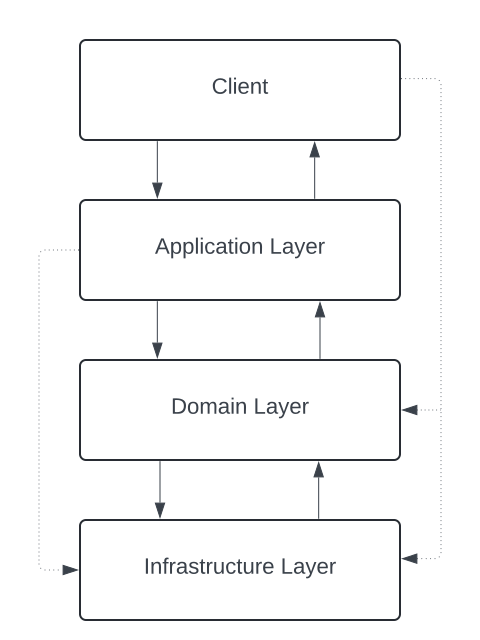
\includegraphics[scale=0.4]{part two/Objektorientierte Analyse/img/layeredarchitecture}
    \caption{Die von DDD propagierte Schicht, bei der die Fachdomäne durch die \textit{Domain Layer} repräsentiert wird, ``the heart of business software`` (\cite[70]{Eva03}). (Quelle: in Anlehnung an \cite[68]{Eva03})}
    \label{fig:layeredarchitecture}
\end{figure}

\noindent
Im Skript\footnote{s. \cite[42]{Wed09b}} beschreibt \textit{Wedemann} die vertikale Schichtenbildung als Abstraktion von der Anwendung, der Hardware, dem Betriebssystem bzw. Virtueller Maschinen als ``\textbf{Layers}``.
Orthogonal dazu gibt es die horizontale Schichtenbildung von Schnittstellen zu den Datenhaltungssystemen (``\textit{Tiers}``\footnote{
\textit{Wedemann} folgt bei der Interpretation von \textbf{Tiers} den Autoren \textit{Alur et al.}: ``A tier is a logical partition of separation of concerns in the system. We view each tier as logically separated from one another.`` (\cite[120]{ACM03})
}), wie \textit{Infrastruktur}, \textit{Domäne}, \textit{Client} (s. Abbildung~\ref{fig:layerstiers})

\begin{figure}
    \centering
    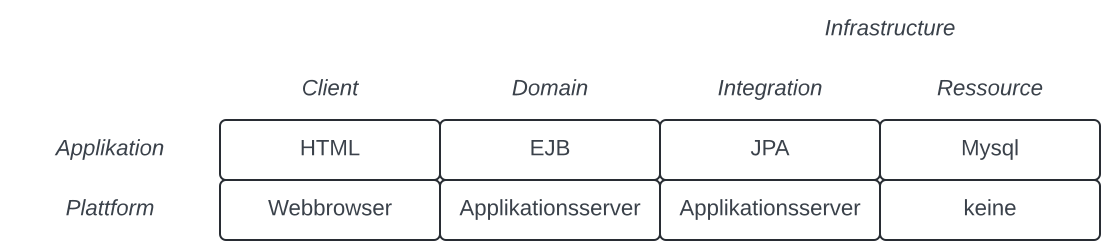
\includegraphics[scale=0.4]{part two/Objektorientierte Analyse/img/layerstiers}
    \caption{Beispiel für eine Schichtenbildung, horizontal wurden die \textit{Layers} gebildet, vertikal die \textit{Tiers}. I.d.R. veranschaulicht eine hierarchische Anordnung der \texbf{Tiers} ihren Kommunikationsfluss besser. Zu der Unterteilung der Infrastrukturschicht in Ressourcen-/Integrationsschicht s.a. \cite[144]{Sta14g} (Quelle: in Anlehnung an \cite[42]{Wed09b})}
    \label{fig:layerstiers}
\end{figure}
